\documentclass[11pt]{article}
\usepackage{amssymb}
%\usepackage{epsfig}
\usepackage{subfigure}
\usepackage{graphicx}
\usepackage{textcomp}
\usepackage{cite}
\usepackage{float}
\makeatletter
\makeatother

\expandafter\let\csname equation*\endcsname\relax
\expandafter\let\csname endequation*\endcsname\relax
\usepackage{amsmath}
\newcommand{\agt}{\mathrel{\raise.3ex\hbox{$>$\kern-.75em\lower1ex\hbox{$\sim$}}}}
\begin{document}

\title{Role of Starvation on Foraging Dynamics}


\author{J. D. Yeakel} \address{Santa Fe Institute, 1399 Hyde Park Road, Santa Fe, New
  Mexico 87501, USA}

\author{S. Redner} \address{Santa Fe Institute, 1399 Hyde Park Road, Santa Fe, New
  Mexico 87501, USA}

\begin{abstract}

  We introduce a minimal model of foraging in which the interplay between
  reproduction and starvation of the foragers, and the regeneration of
  resources, controls the dynamics.  The system consists of a resource that
  renews by logistic growth, as well as two classes of foragers---satiated
  and starving.  Satiated foragers reproduce at a fixed rate and are not
  vulnerable to mortality.  However, a satiated forager can starve when
  resources are scarce; conversely, a starving forager can become satiated
  when the resource is abundant.  Starving foragers do not reproduce and they
  die at a rate $\mu$.  We investigate the dynamics of this system, both in
  the well-mixed (mean-field) limit and by stochastic simulations in two
  dimensions.  For parameters that correspond to a benign environment, the
  system settles into a fixed point.  However, the forager populations
  oscillate in time with an increasing amplitude as the environment becomes
  more harsh.  {\bf needs closing sentence(s).}

\end{abstract}

%\maketitle
\section{Introduction}
%Focus on the tradeoff between REPRODUCTION AND SURVIVAL AS A FUNCTION OF ENERGETIC STATE

Foraging for food (resources) is an essential task of many living
organisms~\cite{B91,OB90,KM01,ASD97,KR85,SK86,Vea96,LKW88,BLMV11}.  Our focus
here is on foraging in an environment where the consumed resource can
regenerate, and with the new feature that the energetic state of the foragers
affects their behavior.  This state---either starving (energetically
deficient) or satiated (energetically replete)---determines how the forager
behaves in this time-dependent environment.  We will specifically investigate
the influence of a forager's energetic state and its reproductive behavior on
the long-time dynamics of the population.  As has been shown in [examples],
individuals that are energetically deficient are unlikely to engage is
reproduction.  Even when such individuals do reproduce, the offspring are
often naturally aborted if there is insufficient caloric resources available
to the parent.  On the other hand, satiated foragers do reproduce, which
thereby exerts increased pressure on resources.  In turn, this can lead to a
population collapse when the resources are subsequently depleted by the
earlier growing population.  Our goal is to understand this interplay between
the foragers' energetic state and environmental resources on the population
dynamics.

In our modeling, foragers look for food by wandering in this changing
environment.  If such a search is successful, the forager is satiated and it
can engage in the essential activity of reproduction.  However, if the search
is unsuccessful for a sufficiently long period, the forager ``starves''.
Such a forager can do nothing else but forage, until it either finds food and
again becomes satiated or it dies when it goes too long without finding
nourishment.  These rules are reminiscent of the ``starving random walk''
model, where a single random walk can take $\mathcal{S}$ steps without
encountering food before starving to death.  Moreover, the resource does not
regenerate, so that the forager ultimately starves to death.  For this
idealized model, it was found that the average lifetime of the forager scales
algebraically with $\mathcal{S}$ in $d\!=\!1$ and $d\!=\!2$ dimensions, and
as $\exp(-A\mathcal{S}^\omega)$ for $d>2$.  Here the exponent
$\omega\approx \frac{1}{2}$ for $d=3$, while $\omega\to 1$ only as
$d\to \infty$, with the latter behavior corresponding to the mean-field
limit.  As we will discuss, regeneration of the resource, together with the
behavioral change between starving and satiated foragers leads to still much
richer dynamical behavior.

We will begin by defining our stage-structured population model that
encapsulates the trade-off between regeneration, reproduction, and
starvation.  We will first explore how the rates of these processes impact
the population dynamics in the mean-field limit, where resources and foragers
are always perfectly mixed.  Under this perfect mixing condition, the species
densities can be described by rate equations, and we will investigate the
dynamical behaviors that arise from these equations.  We will also compare
this continuous rate-equation approach with stochastic simulations that
account for discreteness effects due to the finiteness of the population.
Next, we will extend these stochastic simulations to the physical situation
where the foragers perform random walks in two dimensions.  Intriguing
spatial organization effects arise, in which waves of satiated foragers
reproduce and deplete the environment, followed by satiated foragers
subsequently become starving foragers, many of whom eventually die.  This
allows for a later recovery of the environment and ultimately to repeated
cycles of boom and bust.  As we shall discuss, this quasi-cyclic behavior
arises when the environment is ``stressed'', because the consumption and
reproduction rates are high.  Conversely, for smaller environmental stress,
the system converges to a fixed point.

Finally, we will develop a more general model to understand if there are
common attributes of the dynamics outlined above that have implications
beyond our simple stage-structured model.

\section{The Model}

We incorporate energetics into the model dynamics by assuming that the
foragers can exist in two discrete energetic states---satiated and starving.
Satiated (or full) foragers $F$ are those that have just encountered and
consumed a unit of resource $R$.  On the other hand, a satiated forager that
does not encounter a resource as it wanders is converted to a starving
forager $S$ with rate $\sigma$.  Whenever a forager, either satiating or
starving, encounters resources, one unit of the resource is consumed.  If the
forager was starving, it is recruited into the satiated population with rate
$\rho$.  During the time that a forager is starving, it dies with a fixed
mortality rate $\mu$, while satiated foragers do not experience mortality
risk.  Furthermore, satiated foragers reproduce with rate $\lambda$.
Finally, we assume that, in the absence of foragers, the underlying resource
undergoes logistic growth, with growth rate $\alpha$ and carrying capacity
equal to one.

According to these processes and also under the assumption that the densities
of satiated foragers, starving foragers, and resources (also denoted by $F$,
$S$, and $R$, respectively) are perfectly mixed, they evolve according to the
rate equations:
\begin{align}
  \label{RE}
\begin{split}
\dot F &= \lambda F + \rho  RS - \sigma (1-R)F\,,\\
\dot S &= \sigma (1-R)F - \rho RS - \mu S\,, \\
\dot R &= \alpha R(1-R) -  R(F+S),\\
\end{split}
\end{align}
where the overdot denotes time derivative.

This system of equations admits three fixed points.  Two of them, at
$(F^*\!=\!0,S^*\!=\!0,R^*\!=\!0)$ and $(F^*\!=\!0,S^*\!=\!0,R^*\!=\!1)$
correspond to an environment without foragers.  In this case, the latter
fixed point is stable.  There is also a non-trivial fixed point in which all populations are
represented, $(F^*,S^*,R^*\!>\!0)$, corresponding to an ecologically active
fixed point at

\begin{align}
\begin{split}
F^* &= \frac{\alpha  \lambda  \mu  (\mu +\rho )}{(\lambda +\mu ) (\lambda  \rho +\mu  \sigma )}, \\
S^* &= \frac{\alpha  \lambda ^2 (\mu +\rho )}{(\lambda +\mu ) (\lambda  \rho +\mu  \sigma )}, \\ 
R^* &= 	\frac{\mu  (\sigma -\lambda )}{\lambda  \rho +\mu  \sigma }.
\end{split}
\end{align}

\noindent If this unique fixed point is stable, the species populations
will be globally attracted to it for any set of initial conditions with values greater than zero.

%Linearization
To determine the stability of the non-trivial fixed point, we compute the
Jacobian Matrix $\bf J$, whose elements are given by
$J_{ij}=\partial X_i/\partial X_j$, where $X_i$, with $i=1,2,3$, refers to
the densities $F,S,R$, respectively.  At the non-trivial fixed point, the
Jacobian matrix is
\begin{equation}
\mathbf{J}|_* = 
\left(
\begin{array}{lll}
  \lambda  - \sigma(1-R^*)  & \rho R^* & \sigma(S^*+ F^*) \\
  \sigma(1-R^*) & - \rho R^*-\mu &   -\rho  (S^*+ F^*) \\
  - R^* & - R^* & \alpha(1-2 R^*)-(S^*+F^*) \\
\end{array}
\right).
\end{equation}


Whether the internal fixed point is attracting or repelling is conditioned
on the values of the parameters in the system.  If the parameters of the
Jacobian matrix (at the internal fixed point) are such that its eigenvalues
have negative real values, then it is stable.  The stability of the system
changes if a Saddle-Node bifurcation is crossed, such that a single
eigenvalue obtains a positive real part, defined by the condition
${\rm Det}({\bf J})=0$.  A single Transcritical bifurcation exists at
$\lambda = \sigma$, such that the condition $\sigma < \lambda$ is required for stability of the internal fixed point.

In traditional consumer-resource models, the growth of the consumer scales to both itself as well as the resource.
The reasoning behind this is sound: as the resource density declines, the growth of the consumer is likewise expected to decline.
This dynamic implicitly incorporates the idea that resource depletion lowers consumer growth rates.
However, because we model the effects of starvation by the explicit inclusion of a starving consumer class, we assume that the satiated component of the consumer population has a fixed reproductive rate, which is not dependent on resource density.
Thus, as resource density declines, the recruitment of satiated consumers into the starving class increases, serving to lower consumer growth mechanistically.

Introducing mechanistic starvation imposes an added requirement for the internal fixed point to be stable: the rate of starvation must be greater than the rate of consumer reproduction.
If this is violated, the consumer class reproduces faster than it starves, irrespective of resource density, increasing exponentially.
We suggest that the criterion $\sigma < \lambda$ is in fact biologically reasonable because starvation occurs on a much shorter timescale than reproduction.



% Although a closed-form solution is not possible, a second stability
% condition generally requires $\delta > a \exp \{\frac{b}{c+\epsilon}\}$
% assuming low values of $\mu_x$ and $\mu_y$ (where $a$, $b$, and $c$ are
% some combination of the model parameters), which simplifies to
% $\delta > \frac{\mu_y}{\epsilon}$ when $p=0$.  This condition places a
% lower bound on the consumer's rate of growth as a function of its rate of
% predation on the resource.  As the rate of consumption decreases, system is
% more likely to become unstable if the consumer's rate of reproduction
% declines.

Of additional interest is the existence of parameter regions that permit the
existence of cyclic behavior.  Cycles arise when a pair of complex conjugate
eigenvalues cross the imaginary axis and attain positive real parts.  This
condition is called a Hopf bifurcation, and is defined by
${\rm Det}({\bf S}) = 0$, where $\bf S$ is the Sylvester matrix, which is
composed of the coefficients of the characteristic polynomial describing the
Jacobian matrix.  Although the Hopf condition cannot be solved analytically
for the specific 2-stage model, it can be explored numerically.


\section{Results}

To determine how the consumer-resource system impacted by different rates of starvation, we analyze the systems with respect to $p$.


\section{Discussion}

%The reproductive tradeoff as a strategy



\subsection{Generalized starvation model}
Our conclusions of the mean-field limit starvation model are of course contingent on the functional forms chosen for the birth, death, starvation, and recovery functions.
To expand understanding of the starvation/reproduction tradeoff on stability, we examine a generalization of our model.

To generalize the starvation model, we define the functions controlling reproduction, mortality, and starvation for the original rate equations, such that

\begin{align}
  \label{GE}
\begin{split}
\dot F &= \lambda F + \rho  RS - \sigma (1-R)F = G(F) + H(R,S) - K(R,F)\,,\\
\dot S &= \sigma (1-R)F - \rho RS - \mu S = K(R,F) - H(R,S) - M(S)\,, \\
\dot R &= \alpha R(1-R) -  R(F+S) = P(R) - L(R,S,F).\\
\end{split}
\end{align}

\noindent Although we cannot solve for the fixed points of the generalized model, we can define them as $R^*$, $S^*$, and $F^*$ for the resource, starving consumer class, and satiated consumer class, respectively.
We then define the variables normalized to the fixed point, where

\begin{equation}
r = \frac{R}{R^*},~~~ s = \frac{S}{S^*},~~~\mbox{and}~f = \frac{F}{F^*}.
\end{equation}

By substitution, we can rewrite the general model in terms of normalized variables and functions

\begin{align}
  \label{GNE}
\begin{split}
\dot f &= \frac{G^*}{F^*}g(f) + \frac{H^*}{F^*}h(r,s) - \frac{K^*}{F^*}k(r,f)\,,\\
\dot s &= \frac{K^*}{S^*}k(r,f) - \frac{H^*}{S^*}h(r,s) - \frac{M^*}{S^*}m(s)\,, \\
\dot r &= \frac{P^*}{R^*}p(r) - \frac{L^*}{R^*}l(r,s,f).\\
\end{split}
\end{align}


\noindent where, for example, we use the shorthand $G^* = G(F^*)$.
The normalized general model has the important property that at the fixed point $\dot f = \dot s = \dot r = 0$, then $g(f) = h(r,s) = k(r,f) = m(s) = p(r) = l(r,s,f) = 1$.
This allows us to define the following \emph{scale parameters}. These include those associated with the timescales of the system: $a_f = G^*/F^* + H^*/F^* = K^*/F^*$, $a_s = K^*/S^* = H^*/S^* + M^*/S^*$, and $a_r = P^*/R^* = L^*/R^*$, respectively denoting the turnover time for satiated consumers, starving consumers, and resources.
We also define those scale parameters associated with the branching of biomass through the system, where
$\beta_f = a_f^{-1}G^*/F^*$, which denotes the proportion of gain to the satiated consumer class due to growth (and $1-\beta_f$ is the proportion of gain due to recovery from starvation), and
$beta_s = a_s^{-1}M^*/S^*$, which denotes the proportion of loss to the starving consumer class due to natural mortality (and $1-\beta_s$ is the proportion of loss due to recovery).

The normalized general model can then be written

\begin{align}
  \label{GNE}
\begin{split}
\dot f &= a_f\left[ \beta_f g(f) + (1-\beta_f) h(r,s) - k(r,f)\right]\,,\\
\dot s &= a_s\left[ k(r,f) - (1-\beta_s)h(r,s) - \beta_sm(s)\right]\,, \\
\dot r &= a_r\left[p(r) - l(r,s,f)\right].\\
\end{split}
\end{align}

%A bit on elasticities
%The Jacobian
%The SN/T bifurcation
%The Hopf bifurcation
%Correlation simulations
%What does this tell us?





\begin{figure}[h!]
	\centering
	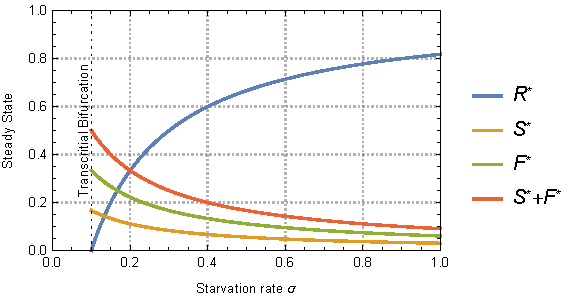
\includegraphics[width=0.5\textwidth]{fig_FP.pdf}
	\caption{
	Fixed points.
	}
	\label{fig_FP}
\end{figure}


\begin{figure}[h!]
	\begin{subfigure}
		\centering
		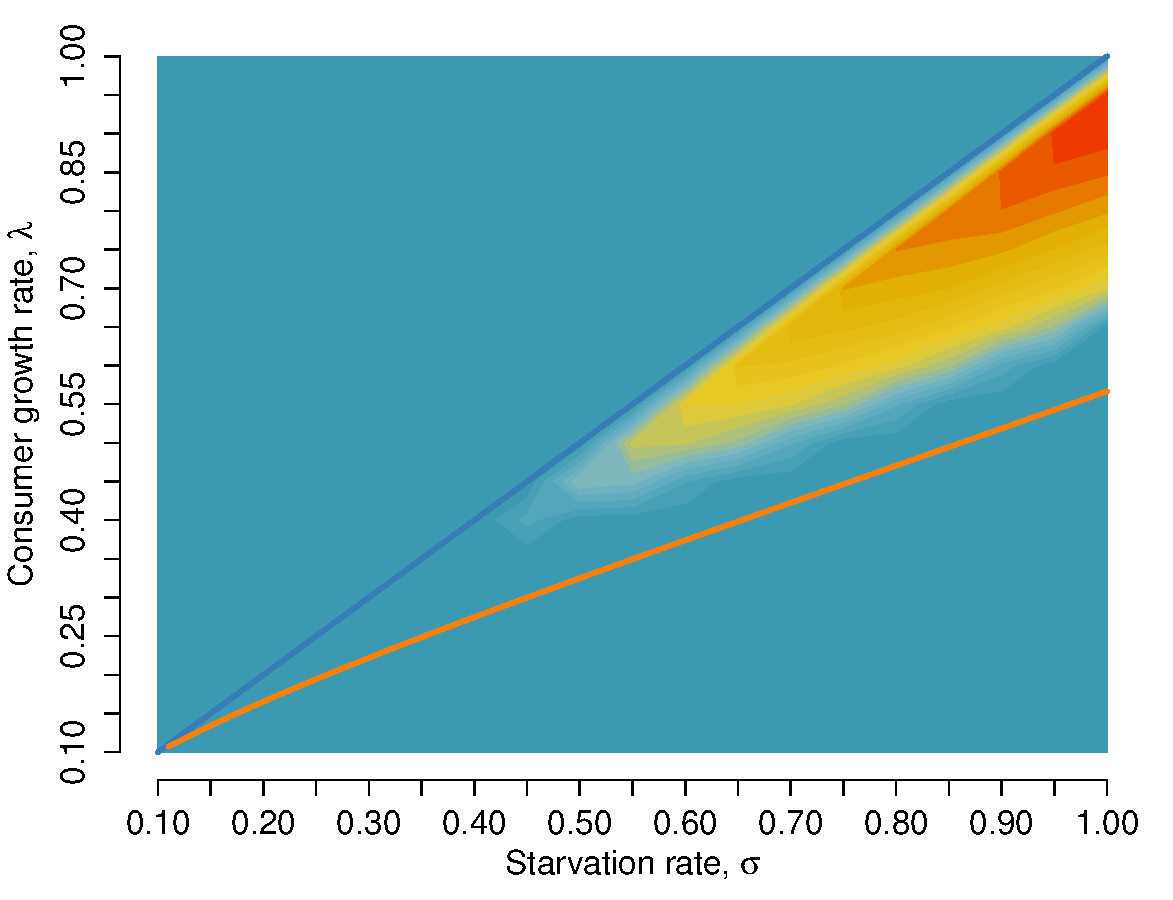
\includegraphics[width=0.4\textwidth]{fig_Hopf.pdf}
	\end{subfigure}
	\begin{subfigure}
		\centering
		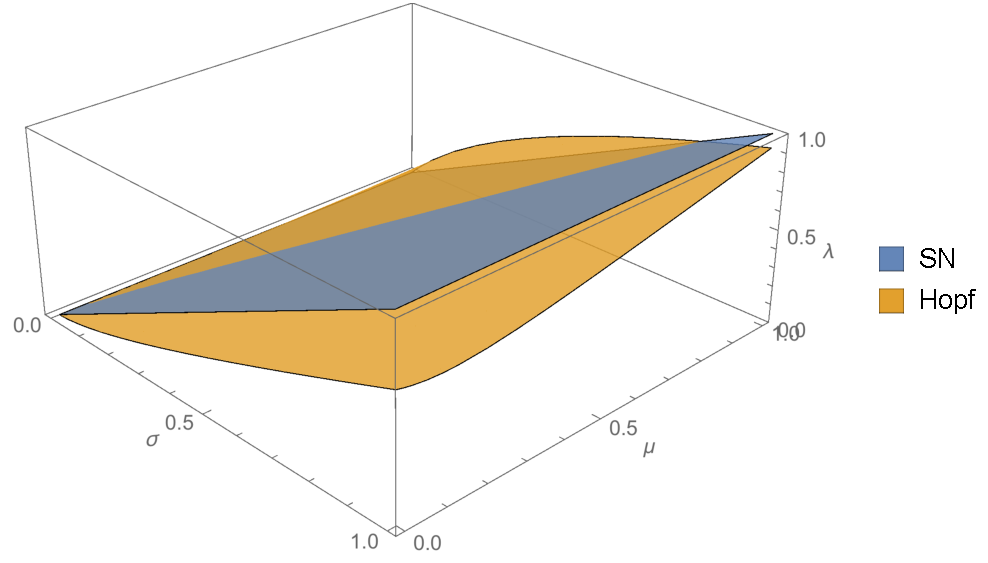
\includegraphics[width=0.4\textwidth]{fig_Hopf3D.pdf}
	\end{subfigure}
	\caption{
		Hopf bifurcation
	}
	\label{fig_Hopf}
\end{figure}



\begin{figure}[h!]
	\centering
	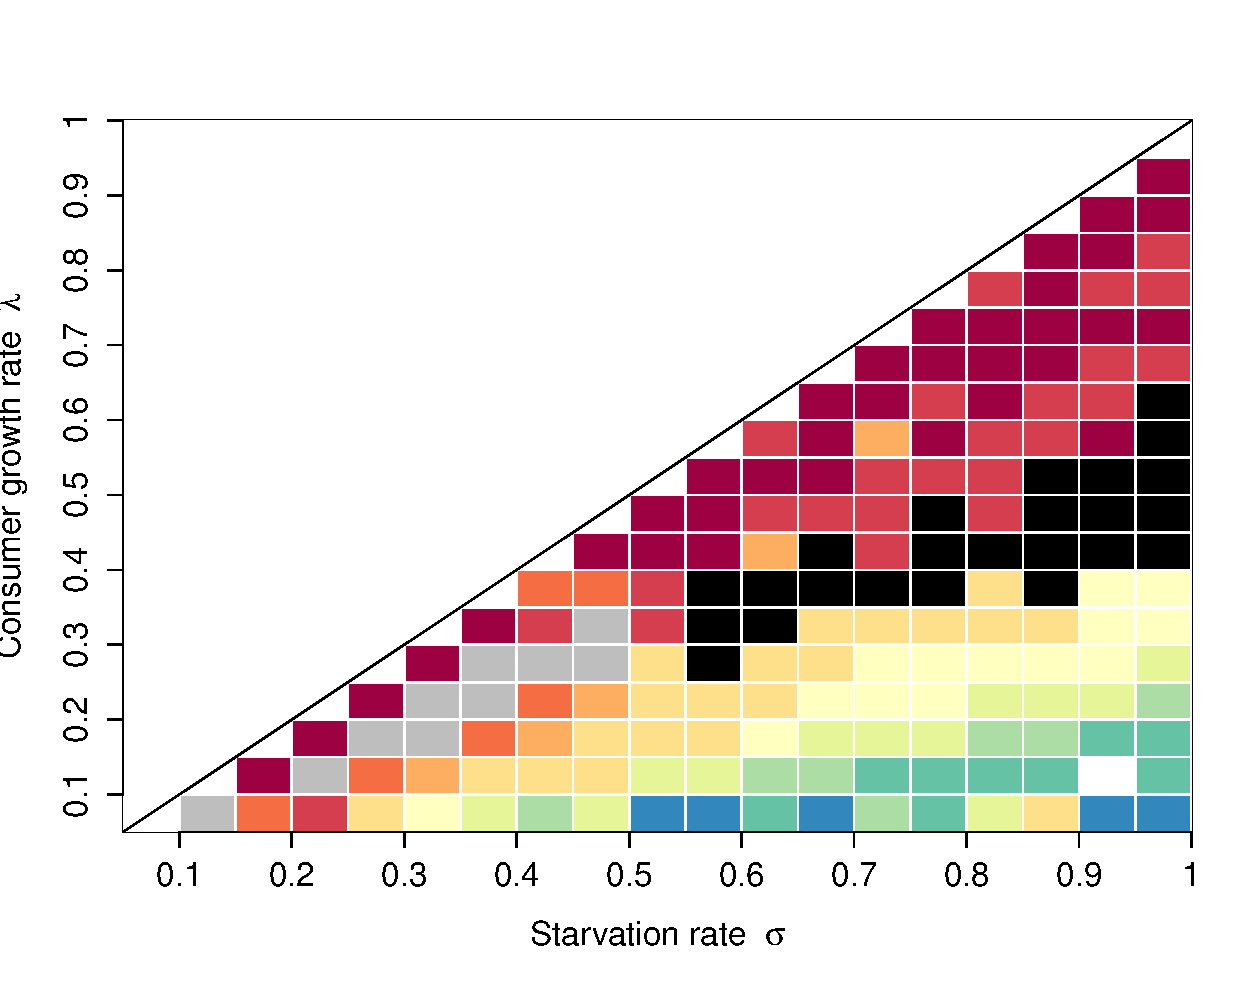
\includegraphics[width=0.5\textwidth]{fig_freqsim.pdf}
	\caption{
	Time series frequencies for spatial simulation model
	}
	\label{fig_FreqSim}
\end{figure}

\begin{figure}[h!]
	\centering
	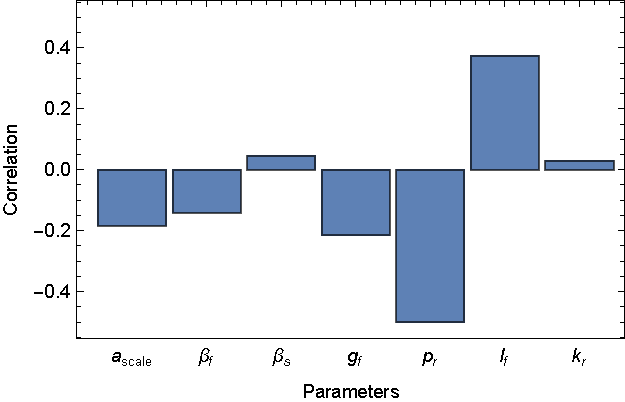
\includegraphics[width=0.5\textwidth]{fig_GenCorr.pdf}
	\caption{
	Generalized modeling results
	}
	\label{fig_Gen}
\end{figure}

JY thanks......  SR thanks NSF Grant No.\ DMR-1205797 (SR) and a grant from
the John S. Templeton Foundation) for partial support of this research.

\newpage

\begin{thebibliography}{99}

\bibitem{B91} J. W. Bell, Searching Behaviour, the Behavioural Ecology of
  Finding Resources, Animal Behaviour Series (Chapman and Hall, London,
  1991).

\bibitem{OB90} W. J. O'Brien, H. I. Browman, and B. I. Evans, Am.\ Sci.\ {\bf
    78}, 152 (1990).

\bibitem{KM01} L. D. Kramer and R. L. McLaughlin, Am.\ Zool.\ {\bf 41}, 137 (2001).


\bibitem{ASD97} J. P. Anderson, D. W. Stephens, and S. R. Dunbar, Behav.\
  Ecol.\ {\bf 8}, 307 (1997).

\bibitem{KR85} P. Knoppien and J. Reddingius, J. Theor.\ Biol.\ {\bf 114}, 273 (1985).

\bibitem{SK86} D. W. Stephens and J. R. Krebs, Foraging Theory (Princeton
  University Press, Princeton, NJ, 1986).

\bibitem{Vea96} G. M. Viswanathan et al., Nature (London) {\bf 381}, 413
  (1996); G. M. Viswanathan et al., Nature (London) {\bf 401}, 911 (1999).

\bibitem{LKW88} M. Levandowsky, J. Klafter, and B. S. White, Bull.\ Mar.\
  Sci.\ {\bf 43}, 758 (1988).
    
\bibitem{BLMV11} O. B\'enichou, C. Loverdo, M. Moreau, and R. Voituriez,
  Rev.\ Mod.\ Phys.\ {\bf 83}, 03 (2011).

\bibitem{R85} S. A. Rice, in Diffusion-Limited Reactions, Comprehensive
  Chemical Kinetics Vol.\ 25, edited by C. H. Bamford, C. F. H. Tipper, and
  R. G. Compton (Elsevier, New York, 1985).

\bibitem{BB76} O. G. Berg and C. Blomberg, Biophys.\ Chem.\ {\bf 4}, 367
  (1976).

\bibitem{GDB14} T. Gueudr\'e, A. Dobrinevski, and J.-P. Bouchaud, Phys.\
  Rev.\ Lett.\ {\bf 112}, 050602 (2014).

\bibitem{T80} M. Tachiya, Chem.\ Phys.\ Lett.\ {\bf 69}, 605 (1980)

\bibitem{BNHW87} R. F. Bonner, R. Nossal, S. Havlin, and G. H. Weiss, J. Opt.\
  Soc.\ Am.\ A {\bf 4}, 423 (1987).

\bibitem{KF00} A. B. Kolomeisky and M. E. Fisher, Physica (Amsterdam) {\bf
    279A}, 1 (2000).

\bibitem{YAL13} S. B. Yuste, E. Abad, and K. Lindenberg, Phys.\ Rev.\
  Lett. {\bf 110}, 220603 (2013).

\bibitem{PW97} M. Perman and W. Werner, Probab.\ Theory Relat.\ Fields {\bf
    108}, 357 (1997).

\bibitem{D99} B. Davis,  Probab.\ Theory Relat.\ Fields {\bf 113}, 501 (1999).

\bibitem{BW03} I. Benjamini and D. B. Wilson, Electr.\ Commun.\ Probab.\ {\bf
    8}, 86 (2003).

\bibitem{ABV03} O. Angel O, I. Benjamini, and B. Virag, Electr.\ Commun.\
  Probab.\ {\bf 8}, 66 (2003).

\bibitem{Z04} M. P. W. Zerner, Probab.\ Theory Relat.\ Fields {\bf 133}, 98 (2005).

\bibitem{AR05} T. Antal and S. Redner, J. Phys.\ A {\bf 38}, 2555 (2005).

\bibitem{W94} G. H. Weiss, \textit{Aspects and Applications of the Random Walk}
(North-Holland, Amsterdam, 1994).

\bibitem{H95} B. D. Hughes, Random Walks and Random Environments (Clarendon,
  Oxford, 1995), Vol. 1.


\bibitem{R01} S. Redner, A Guide to First-Passage Processes (Cambridge
  University Press, Cambridge, England, 2001).

\bibitem{future} O. B\'enichou and S. Redner, unpublished.

\end{thebibliography}



\end{document}
